% This LaTeX was auto-generated from MATLAB code.
% To make changes, update the MATLAB code and export to LaTeX again.

\documentclass{article}

\usepackage[utf8]{inputenc}
\usepackage[T1]{fontenc}
\usepackage{lmodern}
\usepackage{graphicx}
\usepackage{color}
\usepackage{hyperref}
\usepackage{amsmath}
\usepackage{amsfonts}
\usepackage{epstopdf}
\usepackage[table]{xcolor}
\usepackage{matlab}

\sloppy
\epstopdfsetup{outdir=./}
\graphicspath{ {./assignment_code_images/} }

\begin{document}

\begin{par}
\begin{flushleft}
Question: 1.a)
\end{flushleft}
\end{par}

\begin{matlabcode}
load("a4_timeseries.mat");
figure('Position', [10 10 1000 300])

autocorr(vk,'NumLags',400);
xlabel("Lags");
ylabel("ACF");
\end{matlabcode}
\begin{center}
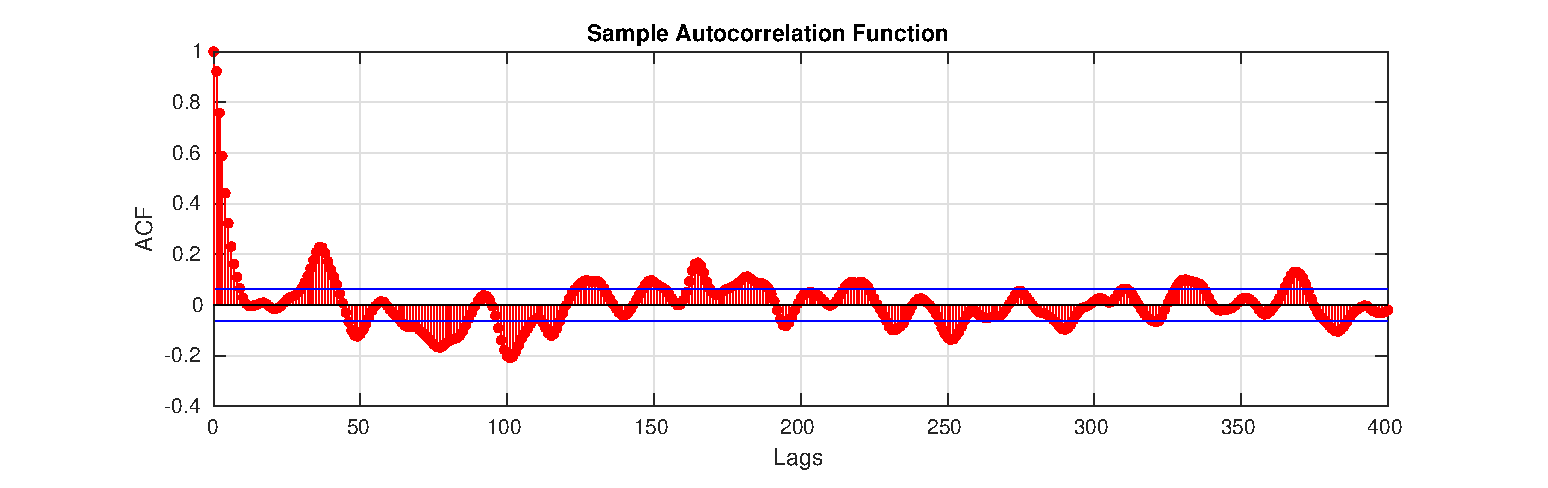
\includegraphics[width=\maxwidth{100.35122930255896em}]{figure_0.eps}
\end{center}
\begin{matlabcode}
parcorr(vk,'NumLags',400);
xlabel("Lags");
ylabel("PACF");
\end{matlabcode}
\begin{center}
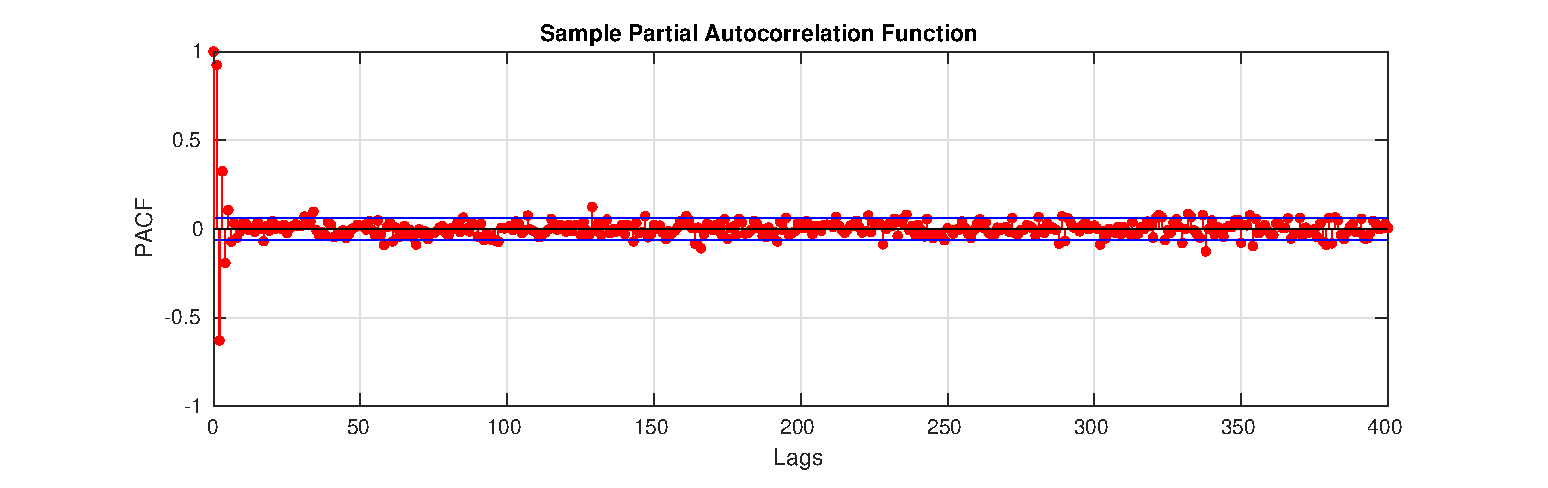
\includegraphics[width=\maxwidth{100.35122930255896em}]{figure_1.eps}
\end{center}
\begin{matlabcode}
parcorr(vk,'NumLags',50);
xlabel("Lags");
ylabel("PACF");
title("Zoomed-in PACF plot")
\end{matlabcode}
\begin{center}
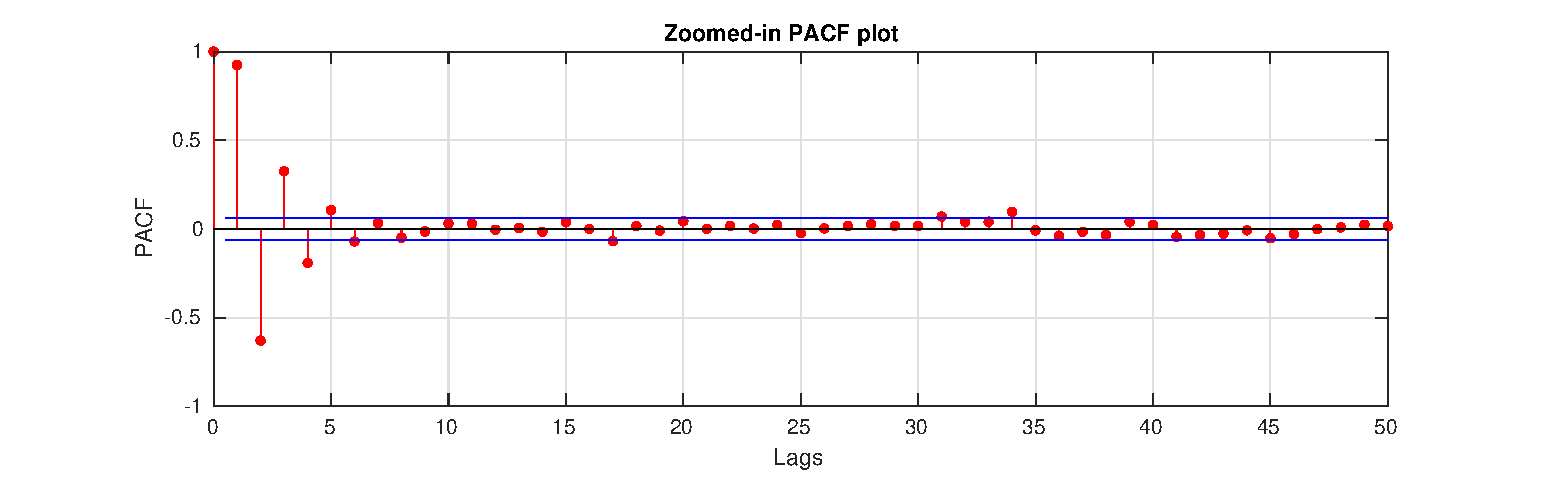
\includegraphics[width=\maxwidth{100.35122930255896em}]{figure_2.eps}
\end{center}

\begin{par}
\begin{flushleft}
Question: 1.b)
\end{flushleft}
\end{par}

\begin{matlabcode}
ar_model = ar(vk,5);
present(ar_model)
\end{matlabcode}
\begin{matlaboutput}
                                                                                                                                                  
ar_model =                                                                                                                                        
Discrete-time AR model: A(z)y(t) = e(t)                                                                                                           
  A(z) = 1 - 1.796 (+/- 0.03149) z^-1 + 1.405 (+/- 0.0639) z^-2 - 0.797 (+/- 0.07362) z^-3 + 0.3823 (+/- 0.06387) z^-4 - 0.1085 (+/- 0.03154) z^-5
                                                                                                                                                  
Sample time: 1 seconds                                                                                                                            
                                                                                                                                                  
Parameterization:                                                                                                                                 
   Polynomial orders:   na=5                                                                                                                      
   Number of free coefficients: 5                                                                                                                 
   Use "polydata", "getpvec", "getcov" for parameters and their uncertainties.                                                                    
                                                                                                                                                  
Status:                                                                                                                                           
Estimated using AR ('fb/now') on time domain data "vk".                                                                                           
Fit to estimation data: 72.73%                                                                                                                    
FPE: 0.9935, MSE: 0.9836                                                                                                                          
More information in model's "Report" property.                                                                                                    
\end{matlaboutput}


\begin{par}
\begin{flushleft}
Question: 3.b)
\end{flushleft}
\end{par}

\begin{matlabcode}
syms w;
gamma = (1/(2*pi)) * (1.68/ (2.5625 - 3.24 *cos(w/2)+ 0.7*cos(w))) * exp(1i*w*l);
acvf_int = int(gamma, w, -pi, pi);

k = zeros(1,15);
acvf = zeros(1,15);
for i = 0 : 15
    k(i+1) = i;
    acvf(i+1) = double(subs(acvf_int,l,i));
end

stem(k,acvf);
\end{matlabcode}
\begin{matlaboutput}
Warning: Using only the real component of complex data.
\end{matlaboutput}
\begin{matlabcode}
ylabel('ACVF')
xlabel('Lags');
\end{matlabcode}
\begin{center}
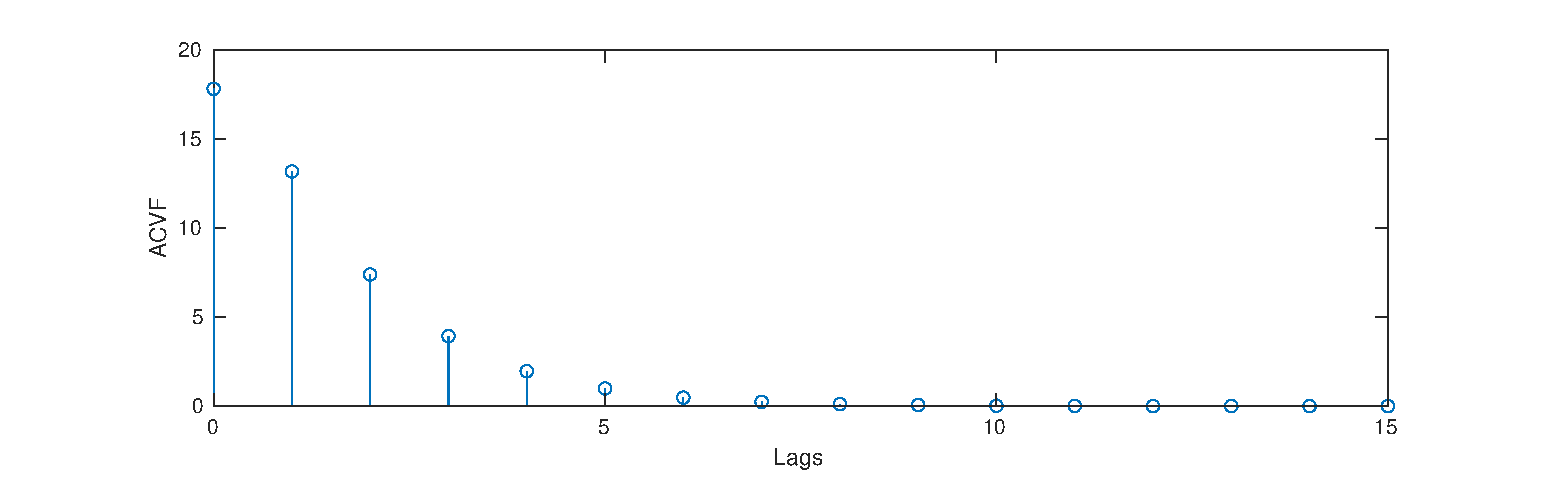
\includegraphics[width=\maxwidth{100.35122930255896em}]{figure_3.eps}
\end{center}

\end{document}
